% !TEX root = main.tex
\chapter{The \lhcb experiment}

Along with \atlas, \cms and \alice, the \lhcb experiment is one of the four major experiments at the European Organisation for Nuclear Research \cern.
The experiment is specialized on precision measurements of the physics processes with \bquark- and \cquark-quarks.
The Large Hadron Collider (\lhc) is briefly described below, followed by a more detailed description of the \lhcb detector and its components (based on \cite{Alves:2008zz}).
At the end of this chapter the \lhcb software stack will be described briefly

\section{The Large Hadron Collider}

\begin{figure}[tbp]
    \centering
    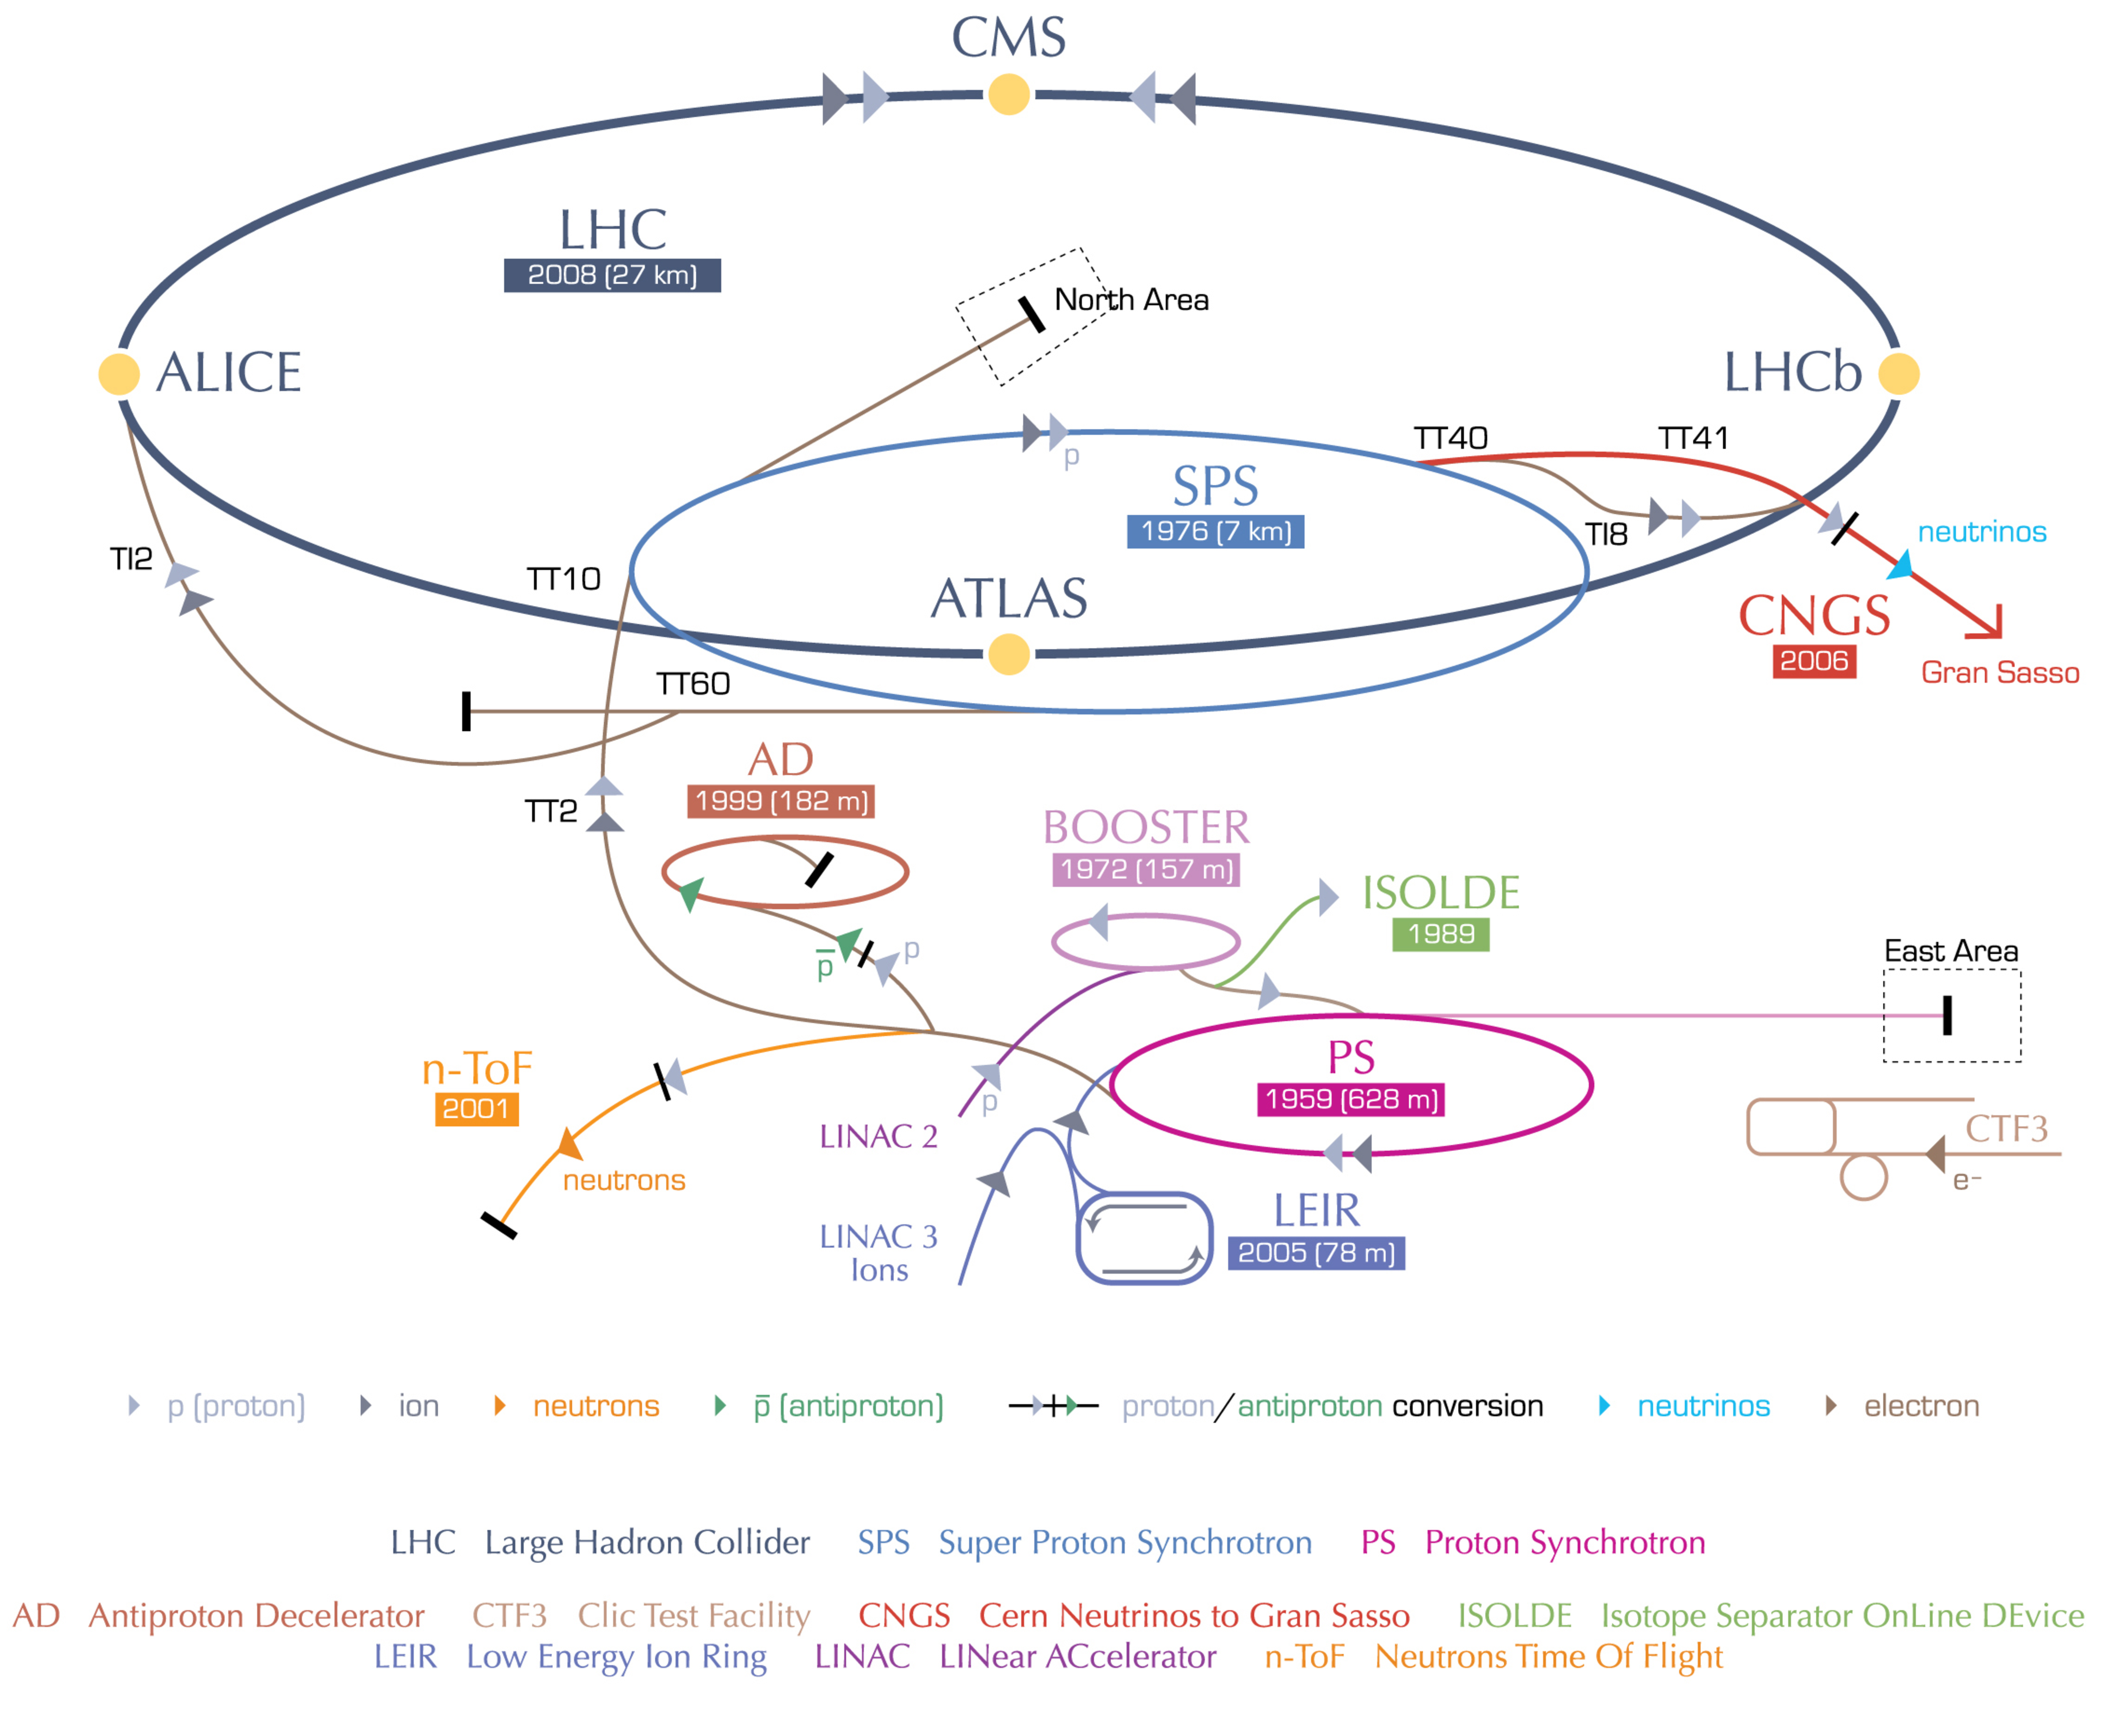
\includegraphics[width=0.75\textwidth]{05lhcb/figs/cern.pdf}
    \caption{Schematic view of the CERN accelerator complex.
    The protons for the LHC are first pre-accelerated to an energy of \SI{450}{\giga\electronvolt} in the LINAC 2, the booster, the proton synchrotron (PS) and the super proton synchrotron (SPS).
    Their path is indicated in the illustration by the light grey arrows~\cite{Christiane:1260465}.}
    \label{fig:CernAccelerators}
\end{figure}
The \lhc is a circular accelerator at \cern near Geneva with a circumference of about \SI{27}{\kilo\metre}.
It is designed to collide protons at a centre-of-mass energy of up to $\sqrt{s} = \SI{14}{\tera\electronvolt}$ at a luminosity of \SI{e34}{\per\cm\squared\per\second}~\cite{Bruening:782076}.
Two proton beams area accelerated in opposite directions and brought to collision at four points.
The first protons in the \lhc were accelerated in \num{2008}.

The \lhc operates in running periods, the first from \numrange{2010}{2012} (Run I), followed by the long shutdown 1 (LS1) in \num{2013} and \num{2014}.
During the Run I the proton beams consisted of about \num{1380} proton bunches, colliding at centre-of-mass energies of $\sqrt{s}=\SI{7}{\tera\electronvolt}$ (\num{2010} and \num{2011}) and \SI{8}{\tera\electronvolt} (\num{2012})~\cite{LHC_statistic}.
For the currently ongoing second running period (Run II) the energy and the number of proton bunches per beam were increased to $\sqrt{s}=\SI{13}{\tera\electronvolt}$ and \SI{2220}{\per\cm\squared\per\second}, respectively~\cite{LHC_statistic}.
The latter was achieved by reducing the bunch spacing from \SI{50}{\nano\second} to \SI{25}{\nano\second}.

Before the protons are injected into the \lhc accelerator ring, they must be pre-accelerated.
This is first done in a linear accelerator, the LINAC 2, followed by the booster, the proton synchrotron (PS) and the super-proton synchrotron (SPS), all of which are circular accelerators.
From the SPS, the protons are then injected into the \lhc ring with an energy of \SI{450}{\giga\electronvolt}~\cite{Bruening:782076} (see \cref{fig:CernAccelerators}).
In order to keep the almost high-energy protons on their circular path, \num{1232} superconducting dipole magnets with a length of \SI{14.3}{\metre} each and a field strength of up to \SI{8.33}{\tesla} are required.

As already mentioned, four major experiments are located at the \lhc.
\atlas and \cms are multi-purpose experiments collecting data at maximum luminosity, \alice mainly studies quark gluon plasmas.
The fourth experiment, \lhcb, performs primarily precision measurements in the field of flavour physics, especially with \bquark- and \cquark-hadrons.
In contrast to the three other experiments, the detector does not cover the entire spatial angle, but is designdes as a forward spectrometer.

\section{The \lhcb detector}

The LHCb detector is a single-arm forward spectrometer with an angular coverage of about \SIrange{10}{250}{\milli\radian}.
The detector geometry is based on the fact that the mainly investigated \bbbar-quark pairs have a high probability of being generated in forward or backward direction (see \cref{fig:anglePlots}).
\begin{figure}[tbp]
    \centering
    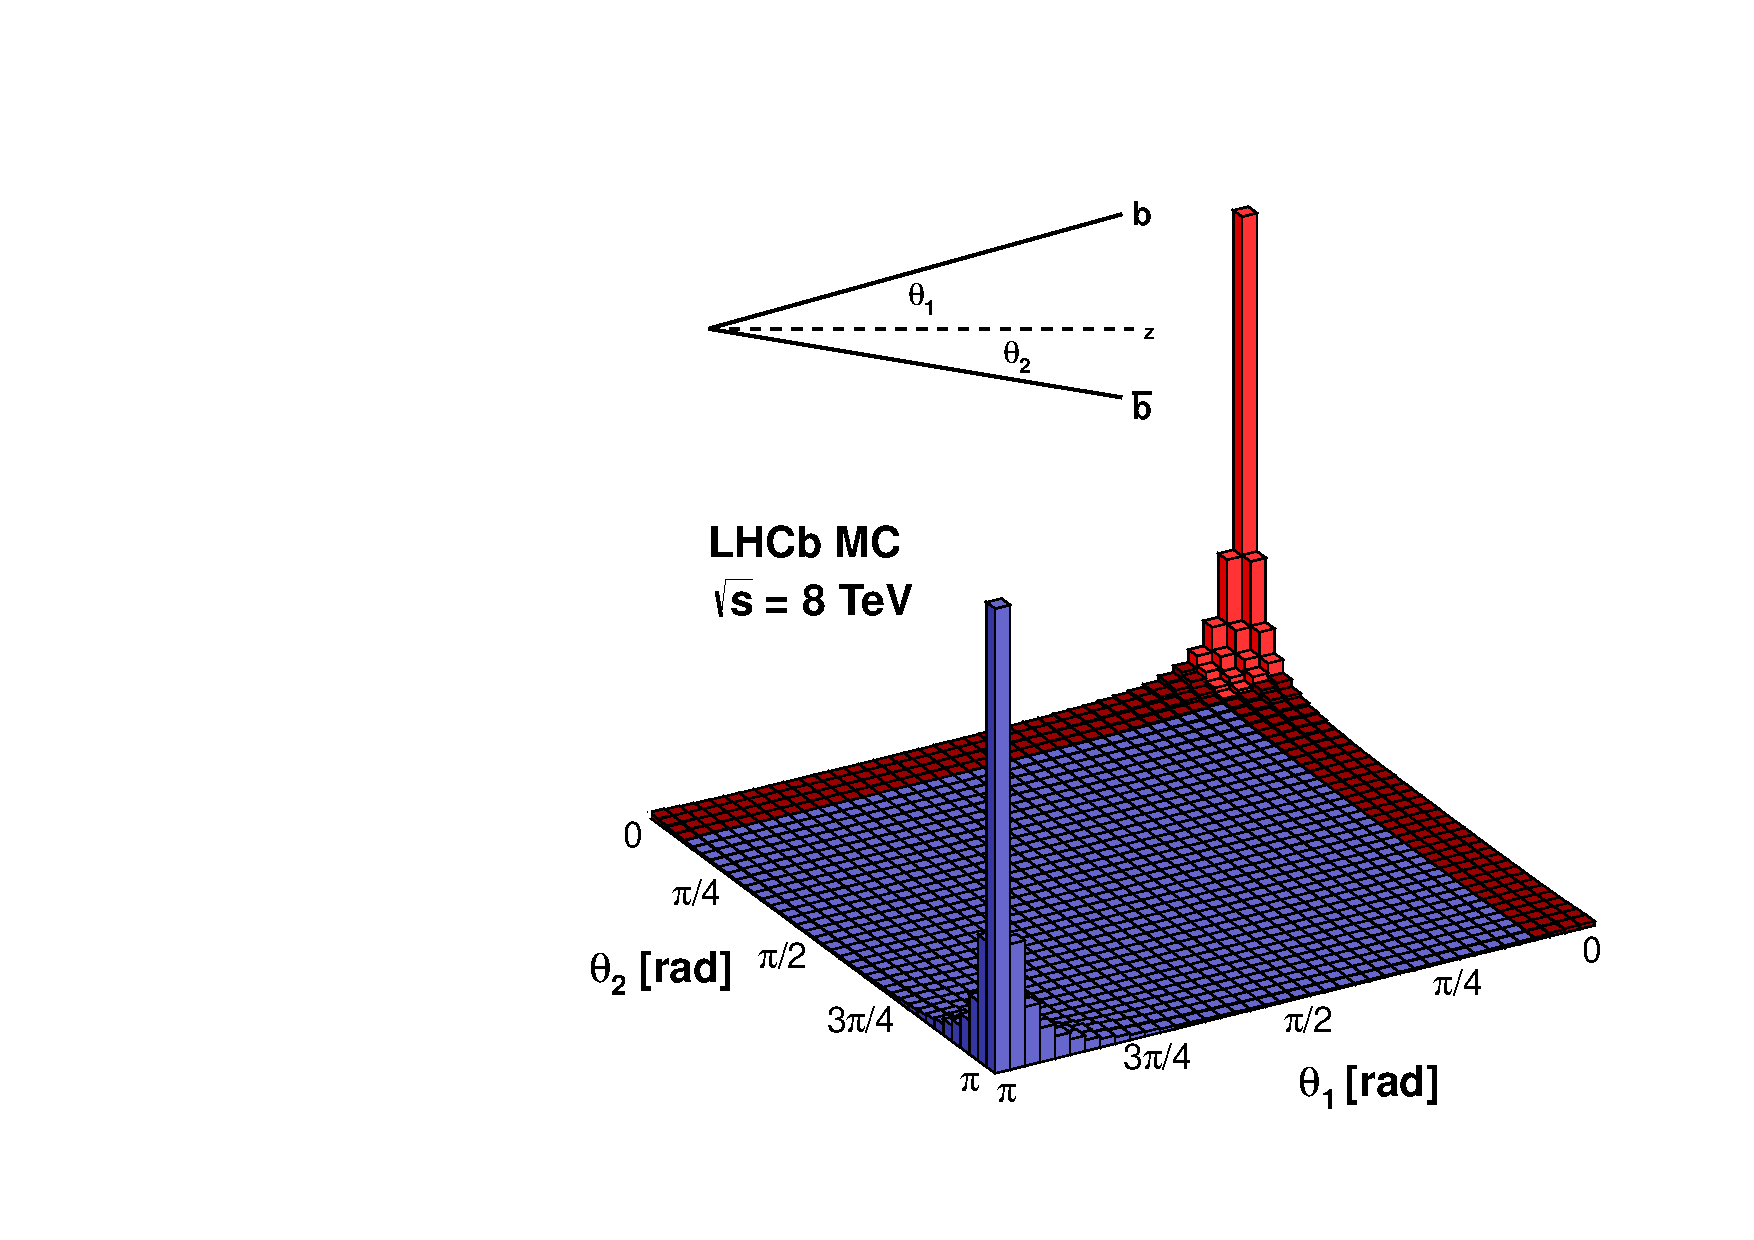
\includegraphics[width=0.4\textwidth]{05lhcb/figs/bbbarCorrelation_angle.pdf}
    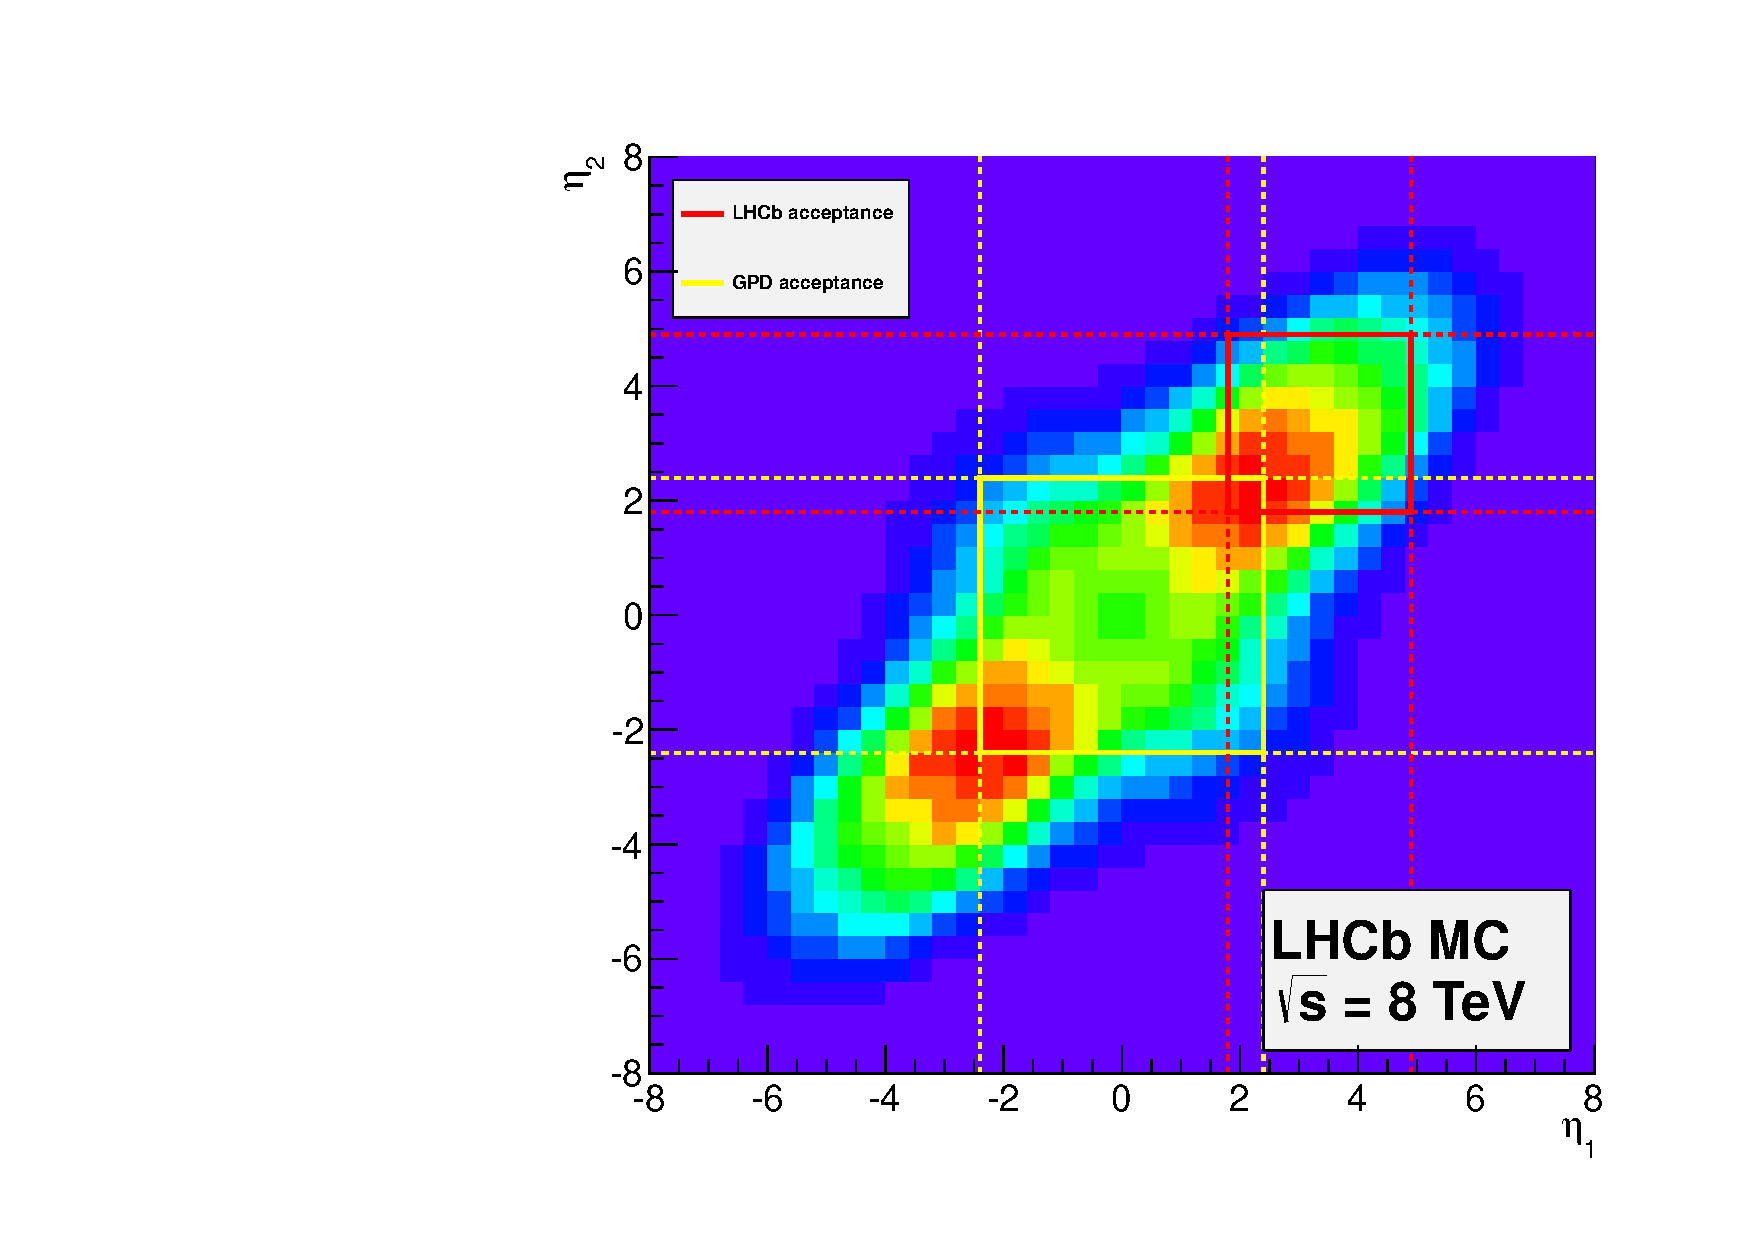
\includegraphics[width=0.4\textwidth]{05lhcb/figs/bbbarCorrelation_rapidity.pdf}
    \caption{Left: Angular distribution of the \bbbar-quark pairs with respect to the beam axis in a proton-proton collision with a centre-of-mass energy of $\sqrt{s}=\SI{8}{\tera\electronvolt}$ as expected from simulations.
    The \lhcb detector acceptance is shown in red.
    Right: Simulated pseudo-rapidity distribution for two \bquark-quarks produced in a proton-proton collision with a centre-of-mass energy of $\sqrt{s}=\SI{8}{\tera\electronvolt}$.
    The yellow box represents the acceptance of a general-purpose detector as \cms or \atlas, the red box shows the \lhcb detector acceptance~\cite{angle_plots}.}
    \label{fig:anglePlots}
\end{figure}
\begin{figure}[tbp]
    \centering
    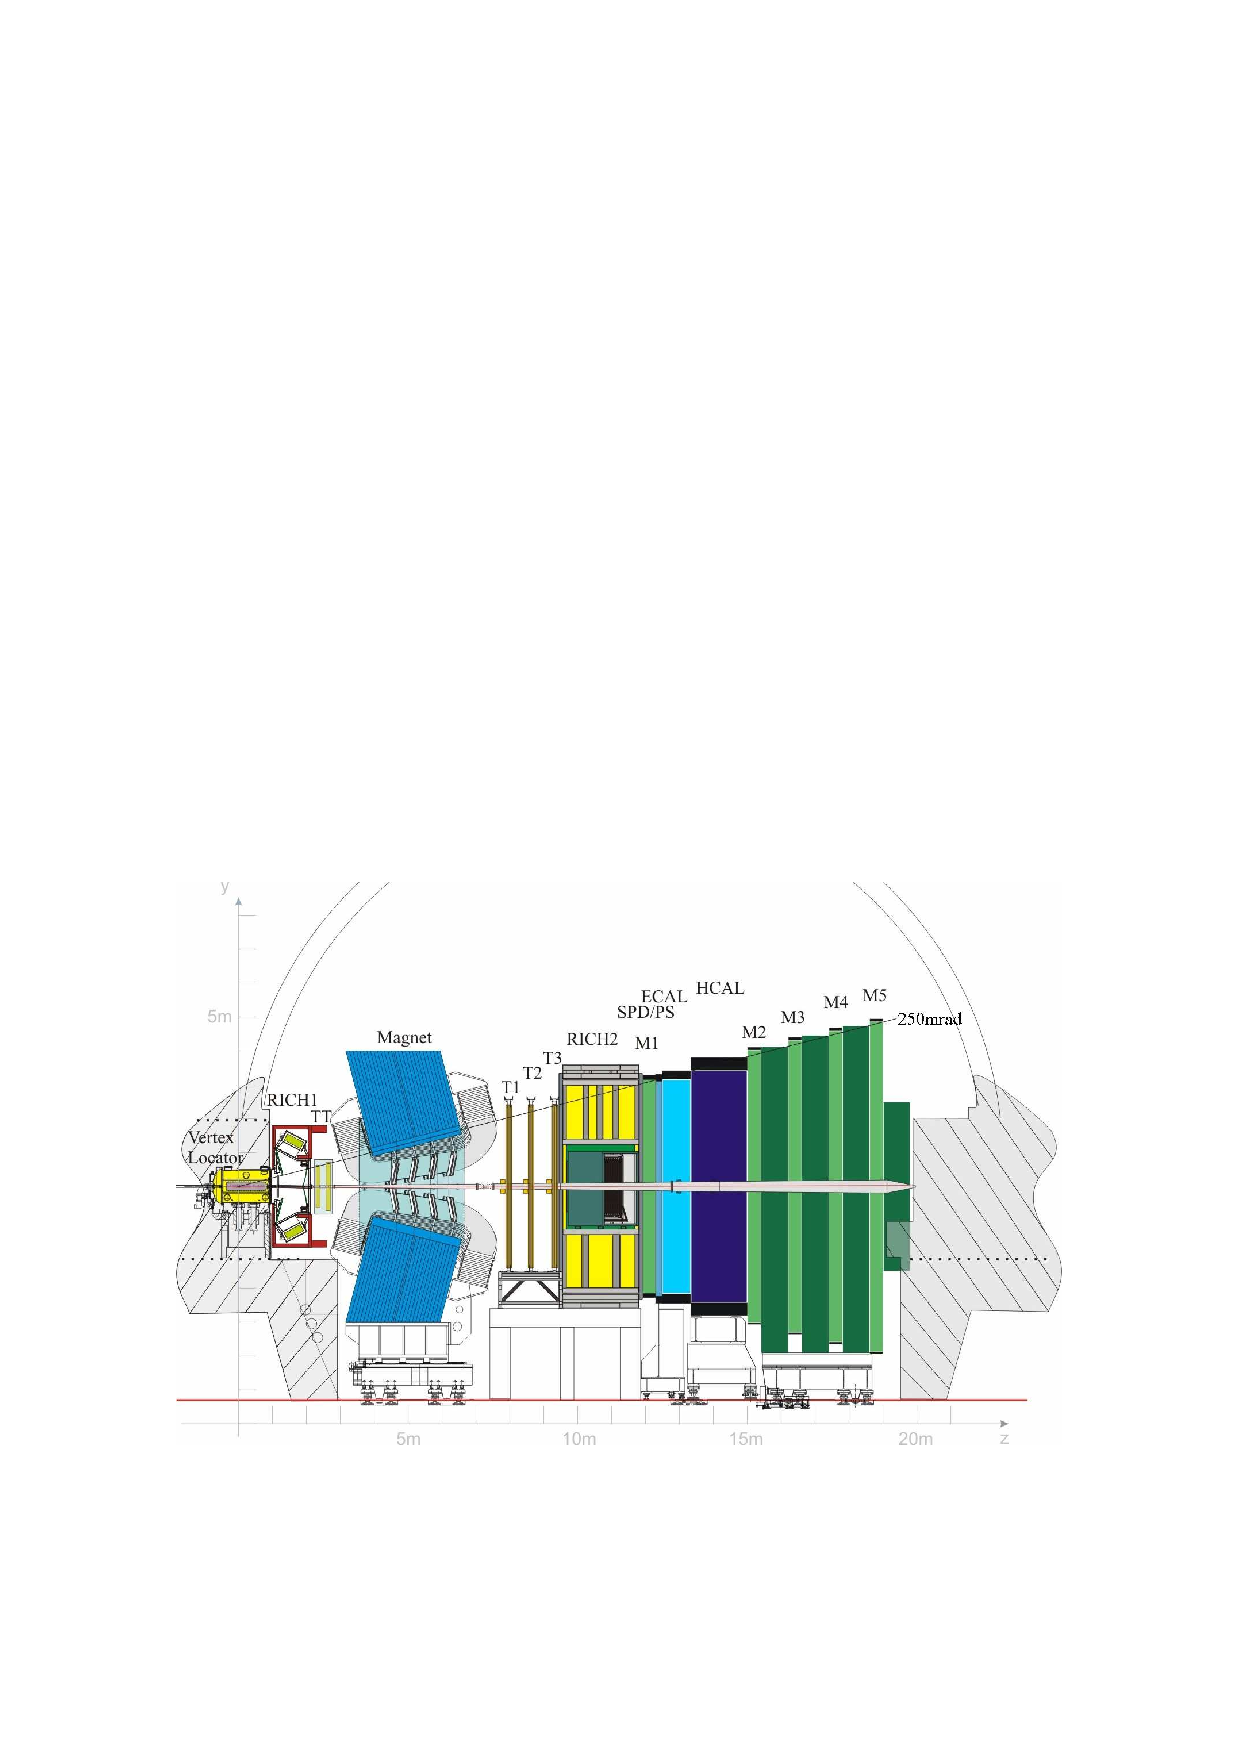
\includegraphics[width=0.8\textwidth]{05lhcb/figs/detector.pdf}
    \caption{Schematic structure of the \lhcb detector: The \velo, the two \rich detectors, as well as the tracking system with magnet, calorimeter and the muon chambers.
    The collision point is located on the left side, enclosed by the \velo~\cite{Alves:2008zz}.}
    \label{fig:lhcbdetector}
\end{figure}
Despite the limited angular coverage, about \SI{25}{\percent} of \bbbar quark pairs are within the detector acceptance.
Furthermore, it is important at \lhcb to resolve individual processes as detailed as possible.
The fewer proton-proton collisions occur simultaneously, the easier this is.
Therefore, \lhcb does not use the maximum luminosity provided by the \lhc, but a constant luminosity of about \SI{4e32}{\per\cm\squared\per\second}~\cite{LHC_statistic}.
This is adjusted by reducing the overlap of the colliding proton bunches at \lhcb compared to the other experiments.
However, since the collision rate with currently \SI{20}{\mega\hertz} is still too high to store all events directly, powerful triggers are also required, which already make an initial selection of the data and receive as many signal end states as possible.
In the following, the individual components of the LHCb detector (see \cref{fig:lhcbdetector}) based on \cite{Alves:2008zz} are explained, separately for the components of the tracking system, the particle identification system and the \lhcb trigger. Though it is important to note, that neither the components described in \cref{sec:tracking} nor the components described in \cref{sec:PartID} are exclusively used for tracking or particle identification purposes, but always a combination of all components is needed for the final reconstruction.

\subsection{The tracking system}
\label{sec:tracking}

The tracking system consists of the \velo, which encloses the collision point, the \ttracker and the tracking stations T1-T3.
Furthermore, a dipole magnet to bend the tracks of charged particles is part of the tracking system.

\subsubsection*{The \velo}
\label{sec:velo}

The vertex locator (\velo) is the detector component closest to the collision point.
It is used to resolve primary and secondary vertices with high precision.
\begin{figure}[tbp]
    \centering
    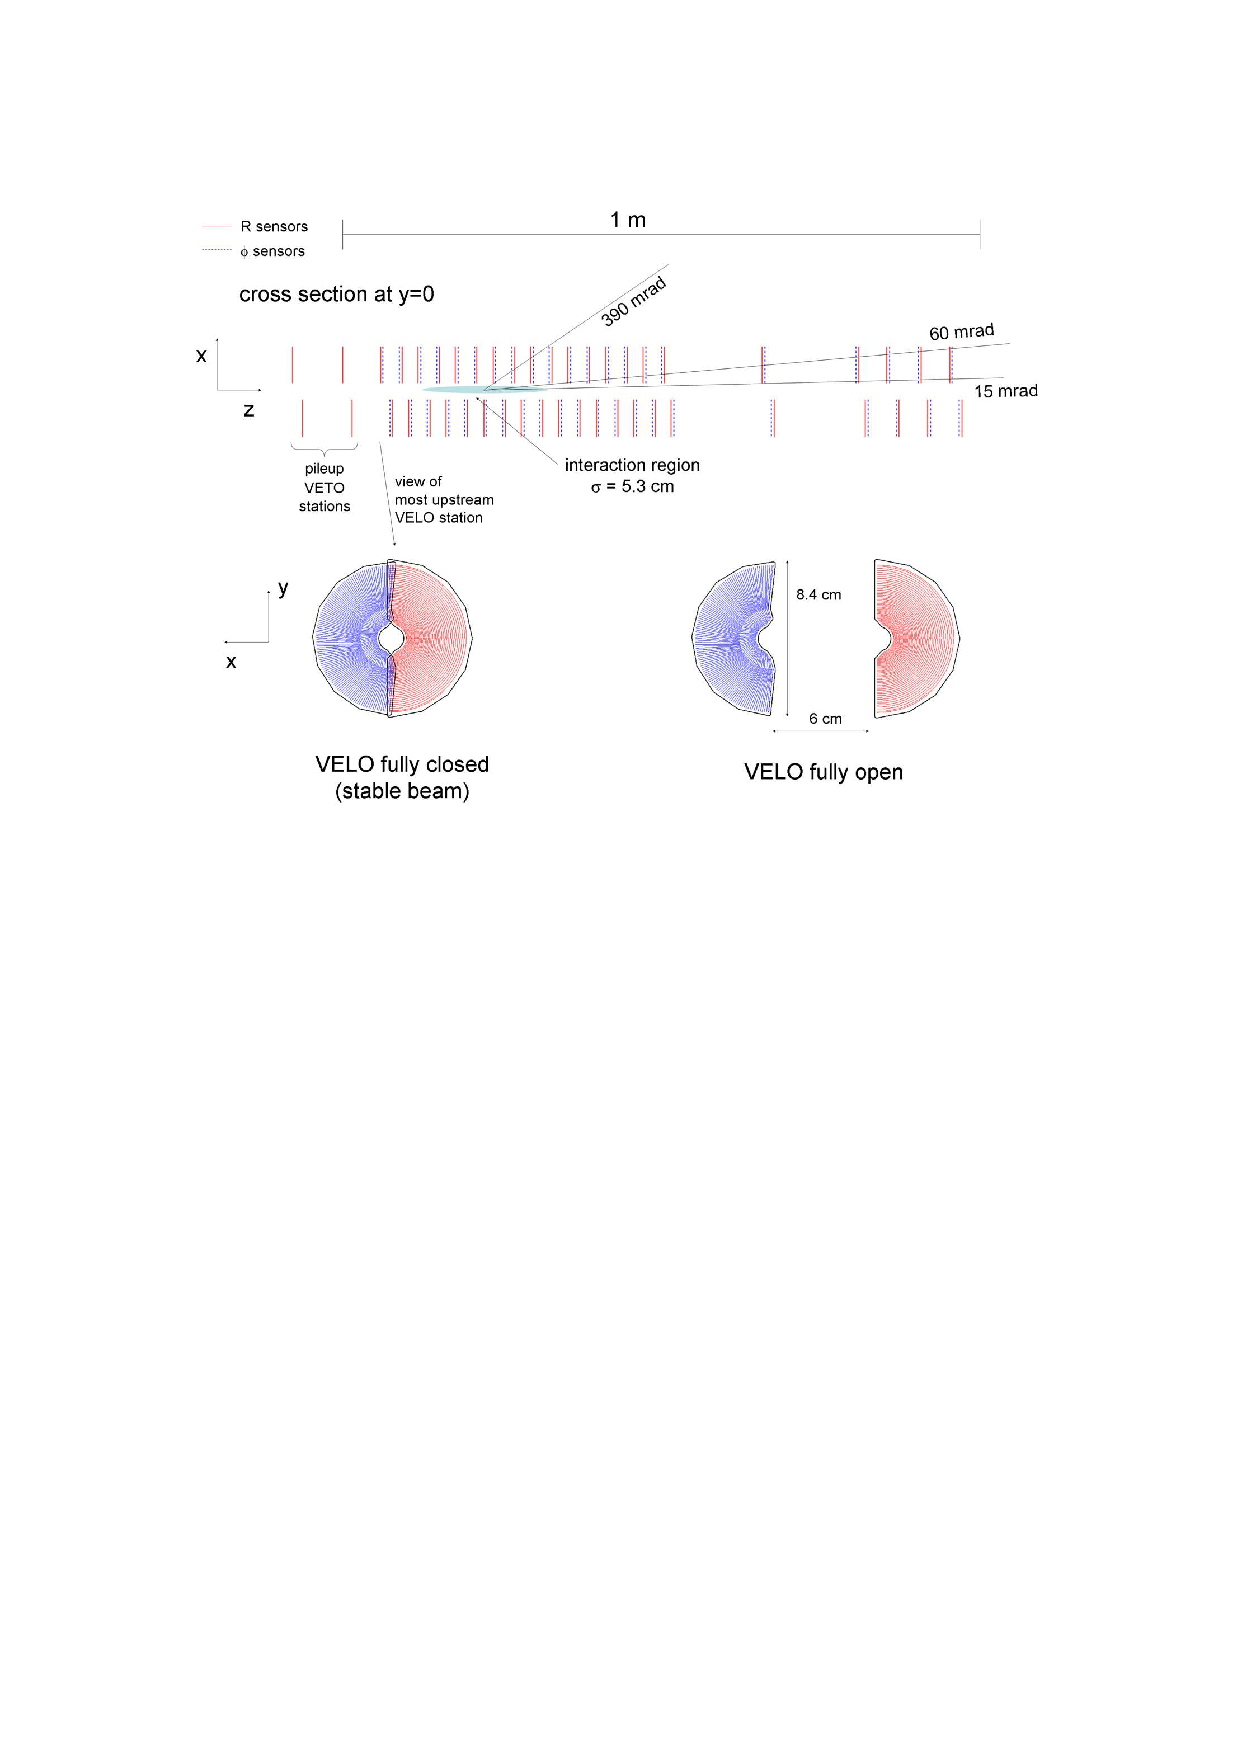
\includegraphics[width=0.8\textwidth]{05lhcb/figs/velo.pdf}
    \caption{Top: View through the $(x,z)$-plane of the \velo at $y=0$ with closed modules.
    Bottom: View from the beam direction onto a module in closed and open state.
    The two halves for $\phi$- (blue) and $r$-measurement (red) can be seen~\cite{Alves:2008zz}.}
    \label{fig:velo}
\end{figure}
The \velo is composed of \num{21} semicircular silicon modules which can be moved up to \SI{8}{\milli\metre} to the beam.
These measure the $r$ and $\phi$ coordinates of the hits left by a transversing particle and are mounted along the beam axis as shown in \cref{fig:velo}.
Furthermore, the inner part close to the collision point of the protons is distinguished from an outer part downstream.

To reconstruct a track for a tranversing particle in the \velo it is required that the particle generates hits in at least three stations.
To achieve an angular acceptance of \SI{300}{\milli\radian} of the \velo under this condition, the distance between the inner stations must not exceed \SI{5}{\centi\metre} with a sensor radius of \SI{42}{\milli\metre}.
If one even requries it under the assumption, that individual modules do not trigger all transversing particles and hence particles must leave hits in four modules, the module distance in the inner part of the \velo has to be \SI{3.5}{\centi\metre}.
An advantage of this small distance is that the mean extrapolation distance from the first measured hit to the interaction point is reduced.

For particles, which are created at $z=\SI{10.6}{\centi\metre}$ downstream of the nominal interaction point, the lower limit of the angular accceptance is \SI{15}{\milli\radian}

To cover full azimuthal acceptance, the two detector halves of each module overlap.
This is possible because the $z$-positions of the respective halves are shifted by \SI{1.5}{\centi\metre} to each other (see \cref{fig:velo}).

\subsubsection*{Tracking stations}
\label{sec:trackingStations}

\subsubsection*{The dipole magnet}
\label{sec:magnet}

\subsection{The particle identification system}
\label{sec:PartID}

\subsection{Trigger}

\section{The LHCb software stack}
